\subsection{Read mapping against reference sequence}
%TODO fastq
%The sequenced reads we obtain from sequencing platform usually are in \textit{FASTQ} format.
%Each record in \textit{FASTQ} file consists of four entries:
%\begin{enumerate}
%  \item read ID, beginning with symbol @
%  \item DNA sequence of read
%  \item symbol +
%  \item \textit{ASCII} encoded quality of each nucleotide in read
%\end{enumerate}

To enable read mapper to efficiently read and process reference sequence, we need to
index reference sequence using mapping software's provided indexing function. Often generated
indexes are incompatible between different read mappers. As a consequence, almost every read
mapping software has their own indexing algorithms.

To perform reference sequence indexing with \texttt{tmap} software, type in linux terminal:\\~\\
\texttt{\refindex{\refSeq}}\\
\texttt{cd ..}\\

%TODO par map1-2-3 pastastit un pateikt rtfm
To perform the actual read mapping against our reference there are availabe six different
mapping algorithms (see \texttt{tmap}'s manual (\url{https://github.com/iontorrent/TS/blob/master/Analysis/TMAP/doc/tmap-book.pdf}.
Some of them are suitable for short reads, some - for longer reads.
In the figure below, histogram of read lengths generated by \IonTorrent~server is shown.
By looking at read length distribution of our sample and it seems that most of
the reads are longer than 150~bp.
\begin{center}
  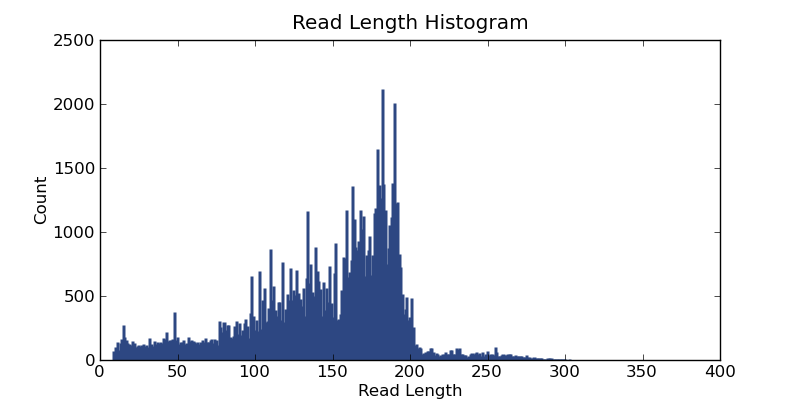
\includegraphics[width=\linewidth, keepaspectratio]{snp_calling/IonXpress_001_rawlib.read_len_histogram.png}
\end{center}
We will choose from one of the algorithms that are suited for longer reads, and
one of such algorithms is \texttt{map3}. To perform the read mapping we need to:
\begin{itemize}
  \item copy reads from \texttt{\textasciitilde/\dataDir} directory to current one
  \item provide it with reference sequence (\texttt{-f \refRel})
  \item provide it with sequencing reads (\texttt{-r \mapReads.fastq})
  \item tell that sequencing reads are in \textit{FASTQ} format (\texttt{-i fastq})
  \item tell that we want alignment to be in compressed \textit{BAM} format(\texttt{-o 1})
  \item tell that we want output to be saved in a file named \texttt{\mapReads\_mapped.bam} (\texttt{-s \mapReads\_mapped.bam})
\end{itemize}
In linux terminal type:\\~\\
\texttt{cd \textasciitilde/\workDir/\reseqDir}\\
\texttt{cp \textasciitilde/\dataDir/\mapReads.fastq .}\\
\tmap{\refRel}{\mapReads.fastq}{\mapReads\_mapped.bam}\\

We have obtained \textit{BAM} file. \textit{BAM} stands for \textbf{B}inary S\textbf{AM} file.
\textit{SAM}, in turn, stands for \textbf{S}equence \textbf{A}lignment/\textbf{M}ap format.

Detailed information about \textit{SAM/BAM} file format, see \url{http://samtools.github.io/hts-specs/SAMv1.pdf}.
\subsubsection{\textit{BAM} file viewing and manipulation}
%Lekcija par bam failu
Let's find out what is in the first 20 lines of \textit{BAM} file using \texttt{samtools} and \texttt{head}:\\~\\
\texttt{samtools view \mapReads\_mapped.bam | head -n 20}\\


To interpret \texttt{FLAG} field (2nd column in \textit{BAM} file), you
can use \texttt{samtools flags} command providing it with the flag you are interested in:\\~\\
\texttt{samtools flags 4}\\

%TODO aprakstīt katru no soļiem
To view \textit{BAM} file header, use 
\texttt{-H} option in \texttt{samtools view} command:\\~\\
\texttt{samtools view -H \mapReads\_mapped.bam}\\

As you can see, we have not defined our read group identifier (\texttt{ID:NOID})
and sample name (\texttt{SM:NOSM}). We can correct it using \texttt{samtools}
command \texttt{reheader}. It takes a \textit{BAM} header and \textit{BAM} file
as input. It replaces \textit{BAM} file's header with the provided header and 
outputs new \textit{BAM} file.

We will read our \textit{BAM} files header and modify it using \texttt{sed}
utility. The modified header will be given to \texttt{samtools reheader}
along with the original bam file. The output will be saved using \texttt{>}
operator:\\~\\
\reheader{\mapReads\_mapped.bam}{\mapReads\_mapped.reheaded.bam}\\

Alternatively, we could have simply defined the read group ID and sample name during mapping process,
using \texttt{tmap}'s option \texttt{-R}:\\~\\% with the complete tab delimited \texttt{RG} line of bam header:\\~\\
\tmapWithRG{\refRel}{\mapReads.fastq}{\mapReads\_mapped.reheaded.bam}\\

%\begin{framed}
%Note that the tab is denoted as \texttt{\textbackslash t} in our header line.
%\end{framed}



We can use \texttt{samtools} command \texttt{tview} to view alignment in a
more human readable format. \texttt{tview} accepts only 
sorted and indexed \textit{BAM} files. Forunately, we can
do this easily using \texttt{samtools} commands 
\texttt{sort} and \texttt{index}:\\~\\
\texttt{samtools sort \mapReads\_mapped.reheaded.bam \mapReads\_mapped.reheaded.sorted}\\
\texttt{samtools index \mapReads\_mapped.reheaded.sorted.bam}\\

\textit{BAM} file indexing allows programs to efficiently access any part of the \textit{BAM} file.
\textit{BAM} index file names usually end with \texttt{.bam.bai}. 

After sorting and indexing, we can view our \textit{BAM} file. In linux terminal type:\\~\\
\texttt{samtools tview \mapReads\_mapped.reheaded.sorted.bam \refRel}\\

Alignment will open in terminal. To get help on viewing alignment, type \texttt{?}.
Type \texttt{q} to quit viewer. A good place to view mapped reads and
test the viewer is \texttt{chr13:27925825}. To go to this position, type \texttt{g}
and enter this coordinate as it is shown.

It is also possible to extract some specific region from the \textit{BAM} file with \texttt{samtools view}
by adding coordinates in form \texttt{chr\textit{N}:\textit{start}-\textit{end}} at the end of command:\\~\\
\texttt{samtools view \mapReads\_mapped.reheaded.sorted.bam chr13:27925800-27925900}\\

To get overall \textit{BAM} file statistics and number of mapped reads for each chromosome, you can use 
\texttt{samtools} commands \texttt{flagstat} and \texttt{idxstats}:\\~\\
\texttt{samtools flagstat \mapReads\_mapped.reheaded.sorted.bam}\\
\texttt{samtools idxstats \mapReads\_mapped.reheaded.sorted.bam}\\

To use these commands, \textit{BAM} file must be sorted and indexed.
%tview chr13:27925825
%region
%idxstats
